Tracking of human bodies in images is a long standing problem in computer
vision research, with a history of prior art beginning as early as the
1970s~\cite{Fischler73, hogg1983model}. The wide variety of important
applications that rely on accurate and stable estimates of human pose has been
a strong motivator for much of this research. Perhaps chief among these
applications has been motion capture for the entertainment industry, where
human body localization and pose inference enables accurate reconstruction and
re-targeting of animation data to synthetic computer generated models. It is
therefore not surprising that a large portion of the literature relates to
\emph{marker-based} motion capture, with a specific focus on capturing
realistic skeletal animation data. Furthermore, many commercial solutions exist
for \emph{marker-based} motion capture, such as those from Vicon and Optitrack,
which are able to predict marker location within sub-millimeter accuracy and at
very high frame-rates (up to a few thousand hertz).

However, there are many applications that require accurate tracking of humans
in images without the use of adding visual annotations or markers.
Human-Computer-Interaction (HCI), virtual reality, surveillance, gait analysis,
medical diagnosis applications, biometrics, action recognition and many other
applications are examples where existing \emph{marker-based} motion capture
solutions are often inappropriate or infeasible. Furthermore, recent
applications in HCI demand real-time performance which has proven to be a
particularly difficult constraint, especially for solutions using only
RGB-based capture devices. Targeting real-time and low-cost applications for
human pose estimation, this work focuses on human body localization without the
use of visual annotations - so called \emph{marker-less} motion capture.
Furthermore, this thesis explores solutions of the localization problem that
make use of only one camera view (or monocular capture) as this is the lowest
barrier of entry for wide-spread use. While calibrated multi-camera capture
rigs are feasible for off-line applications, the ubiquity of single RGB and
depth cameras (in devices such as laptops and cell phones) make this input
modality an appealing research framework.

\begin{figure}[ht]
\centering
	\subcaptionbox{\footnotesize Shape \& Clothing Variation\label{fig:difficult_a}}{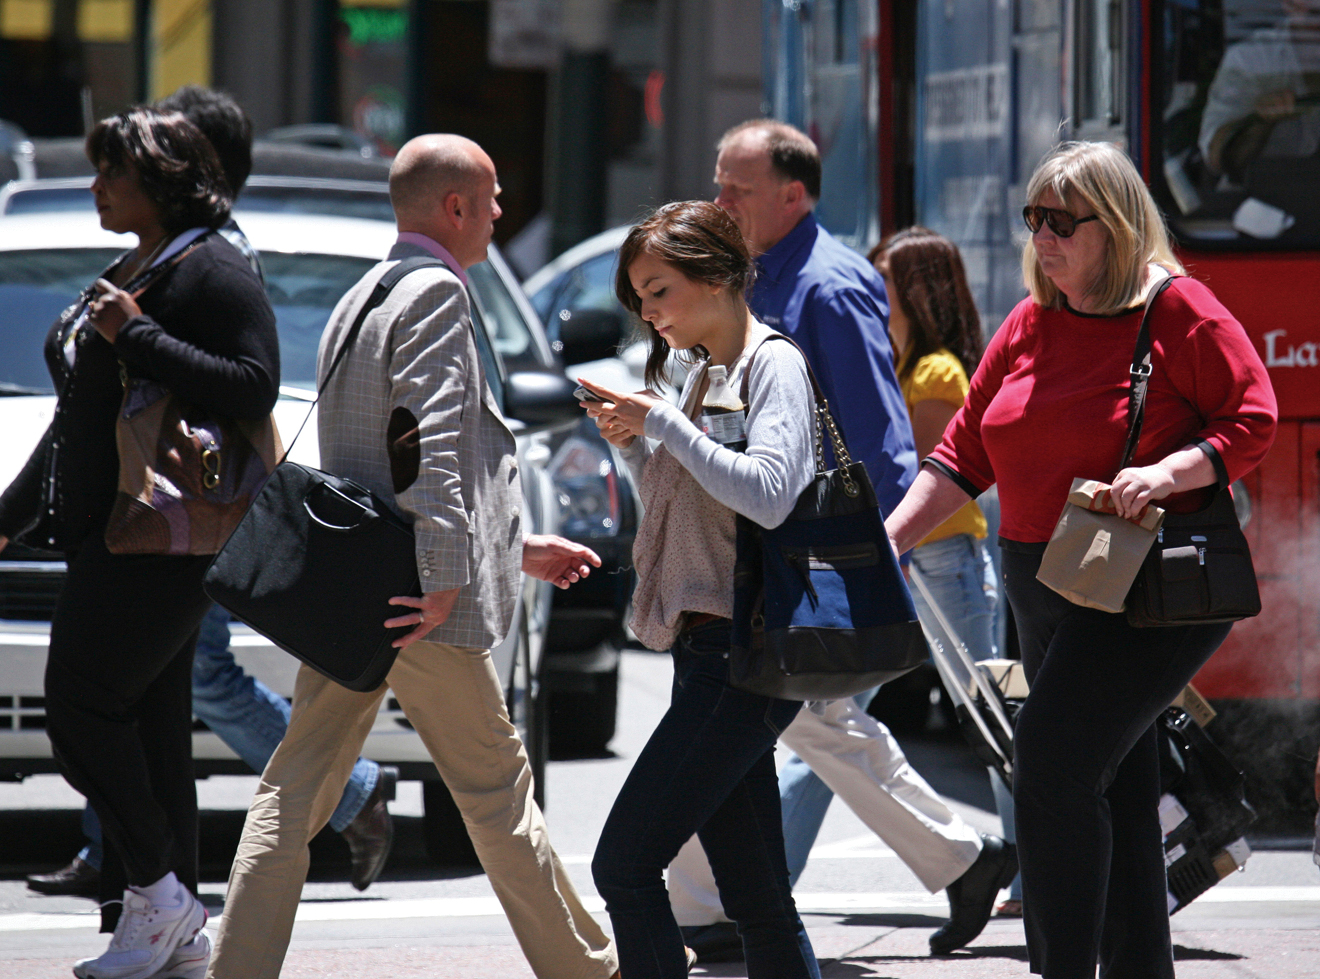
\includegraphics[height=3.9cm]{figures_introduction/pedestrian}}
	\subcaptionbox{\footnotesize Lighting Variation\label{fig:difficult_b}}{
\includegraphics[trim=1.7cm 1.0cm 1.5cm 0.5cm, clip=true, height=3.9cm]{figures_introduction/yoga-pose}}
	\subcaptionbox{\footnotesize Self Occlusion\label{fig:difficult_c}}{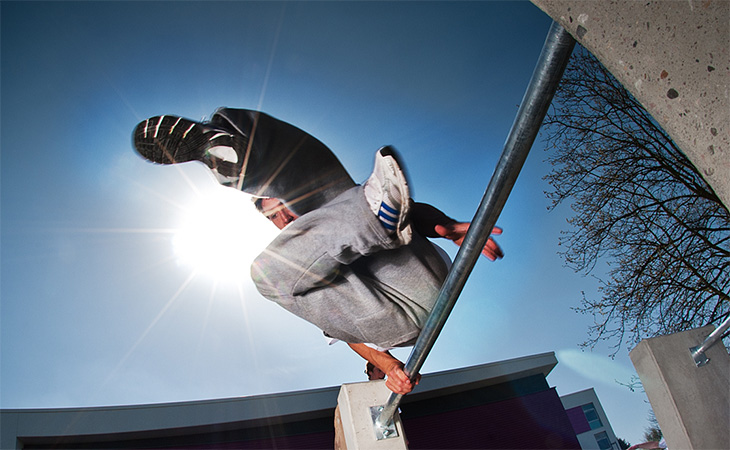
\includegraphics[trim=3.0cm 0.0cm 6.5cm 2.0cm, clip=true, height=3.9cm]{figures_introduction/x-move_parkour_.jpg}}
        \caption{Difficult Samples for Human Body Pose Recognition}
        \label{fig:difficult}
\end{figure}

Human body localization is complicated and difficult for numerous reasons, and
some difficult examples are shown in Figure~\ref{fig:difficult}. As with many
computer vision applications, the high dimensional nature of the image input
makes inferring the low-dimensional pose representation difficult since the
input dimensionality cannot be easily enumerated. However, unlike many classic
computer vision tasks, human body tracking also involves localizing body parts
that undergo large amounts of deformation and exhibit wide variation in both
body-shape and appearance. Deformation increases the intrinsic input
dimensionality of the space of possible poses and furthermore leads to
occlusion, which means that pose inference must be performed with potentially
missing data. Appearance variation can be the result of clothing, lighting
variation or the subjects age or gender; therefore any inference solution must
learn invariance in order to provide a stable estimate of pose under such
wildly varying conditions. Lastly, large and comprehensive datasets exist for
image classification tasks~\cite{deng2009imagenet}, however human-body pose
datasets are many orders of magnitude
smaller~\cite{modec,andriluka14cvpr,Johnson10}. The lack of a comprehensive
standard dataset has traditionally made training robust discriminative
architectures difficult as such networks are prone to over-training when the
training set sizes are limited.

Despite these significant challenges, this work will present a framework for
human body pose localization that offers a significant improvement over
existing traditional architectures. The basis for all the tracking solutions
presented in this thesis is the use of Convolutional Networks (ConvNets), which
have seen a recent surge in success and popularity due to advances in Graphics
Processing Unit (GPU) hardware as well as new and improved techniques for
training them. ConvNets are biologically inspired variants of multi-layered
perceptrons, which exploit spatial correlation in natural images by extracting
features generated by localized convolution kernels. In the context of object
detection, the use of fully convolutional networks result in trained detectors
which are invariant to translation, and this work makes heavy use of this
feature for the architectures presented in Parts \ref{part:two},
\ref{part:three} and \ref{part:four}. A full-review of ConvNets - specifically
their formulation and training via the Back-Propagation algorithm - is outside
the scope of this thesis and interested readers should refer to
\cite{reading_list} for an overview of seminal literature.

ConvNets have been used successfully to solve many difficult machine learning
problems: image classification~\cite{pedestrianCVPR13, overfeatSermanet,
ImageNet_NIPS2012_0534, googlenet}, scene understanding~\cite{Farabet}, video
analysis~\cite{KarpathyCVPR14} and natural language
processing~\cite{ilya_sequence,cho_emnlp_2014}. Likewise, they have recently
out-performed all existing models on the task of hand-pose
recognition~\cite{tompsonTOG14} using an depth camera source, and monocular
human-body pose recognition using an RGB camera~\cite{tompsonnips2014,
arjunaccv2014, jainiclr2014, deeppose, chennips2014, tompson_efficient}. In
this work, we will present our results for the current state-of-the-art models
(at time of writing) for human body and hand pose recognition.

\subsection*{Thesis Outline}

This thesis will explore solutions to two difficult computer vision problems
related to the localization of humans in images: 1) monocular hand-pose
recognition from depth images and 2) monocular full body-pose recognition from
RGB images. This exploration will cover four primary publications
\cite{tompsonTOG14}, \cite{tompsonnips2014}, \cite{arjunaccv2014},
\cite{tompson_efficient} in Parts \ref{part:one}, \ref{part:two},
\ref{part:three} and \ref{part:four} respectively. Within each part, the first
section will define the specific problem and present an overview of the
architecture. The second section will present the model and any algorithmic
details necessary to repeat experiments. Then the final solution will present
experimental results, compare our work with previous state-of-the-art and
describe any limitations.

\subsection*{Summary of Contributions}

The following is a summary of the major contributions of this thesis:

\begin{itemize}

\item In Part~\ref{part:one} we describe a novel pipeline for both offline
ground truth dataset creation, as well as real-time pose-detection of human
hands in depth video. While Neural Networks have been used for pose detection
of a limited set of discrete hand gestures (for instance discriminating between
a closed fist and an open palm)~\cite{nagi,nowlan}, to our knowledge this is
the first work that has attempted to use such networks to perform dense feature
extraction of human hands in order to infer continuous pose.

\item In Part~\ref{part:two} we describe a novel ConvNet architecture which
combines a traditional sliding-window based part detector with a Graphical
Model. We describe a graphical model formulation which is inspired by standard
MRF belief propagation, which can be trained jointly with a standard
deep-learning architecture to improve detection performance. At the time of
writing, this model is the state-of-the-art model for the FLIC~\cite{modec},
LSP~\cite{Johnson10} and MPII~\cite{andriluka14cvpr} datasets.

\item In Part~\ref{part:three} we show that simple motion features can be used
to significantly improve the performance of traditional ConvNet architectures.
To our knowledge, this was the first work to empirically examine the impact of
multi-frame inputs to ConvNets in the application of pose detection.

\item In Part~\ref{part:four} we examine the issue of localization accuracy
degradation in ConvNet architecture due to spatial-pooling layers. We present a
novel cascaded architecture, that makes use of shared features, in order to
improve localization accuracy while maintaining runtime performance. We are the
first to show that a ConvNet trained to infer the 2D pose of humans in images
is able to be competitive with - and in some cases out-perform - humans trained
on the same task.

\end{itemize}
